\section{Cyclus}
The Cyclus \gls{NFCS} framework and its
modeling ecosystem, the suite of agents and other
physics plug-in libraries compatible with it, incorporate
modern insights from simulation science and software
architecture \cite{huff_fundamental_2016}. Cyclus
has a multitude of benefits from other available
\glspl{NFCS} codes - open-sourceness, modularity,
and extensibility. Its agent-based modeling approach
is ideal for modeling coupled, physics dependent
supply chain problems common in \glspl{NFC}.
The framework allows for dynamic loading of 
external libraries, which allow the users to plug-and-play
different types of physics models for their \gls{NFC}
simulation.

\subsection{Open Source}
License agreements and institutional
approval is need for most \glspl{NFCS} like COSI, DANESS, DESAE, EVOLCODE,
FAMILY21, NFCSim, ORION and VISION \cite{juchau_modeling_2017}, making
it hard for both the usage and development in an academic setting.
On the other hand, Cyclus relies completely on open source,
free libraries, allowing all users to both use and develop the
Cylcus framework and existing libraries. The open-sourceness
of Cyclus encourages collaboration - any user can propose
improvements or provide input for Cyclus.

\subsection{Modularity and Extensibility}
In most modern \glspl{NFCS}, the facilities and their
behavior (and its fidelity) is confined in the software.
Also, most modern \glspl{NFCS} are restricted to model
a set of fuel cycles (once-through, continuous reprocessing)
with restrictions to connections between facilities. On the
other hand, Cyclus allows users to plug-and-play different libraries
that contain different fidelity modules within the Cyclus framework
(shown in figure \ref{fig:core}).
Also, the Cyclus simulation relies on a market-based model
for material trades between facilities, so the user can design
any novel fuel cycle. Also, this gives Cyclus the option to not
be limited to nuclear fuel cycles, but any system analysis
involving multiple connected facilities with physics-based
calculations.


\begin{figure}[htbp!]
	\begin{center}
		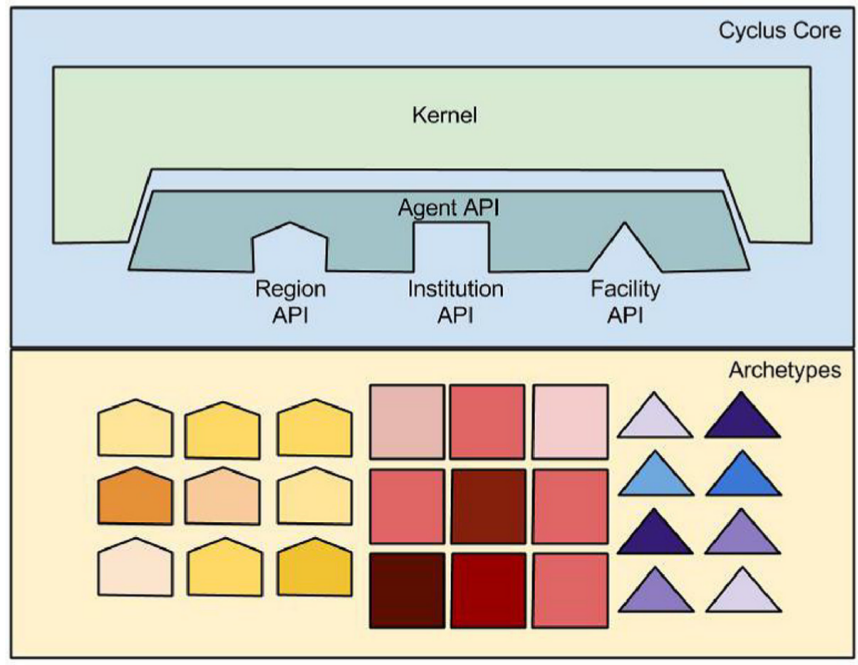
\includegraphics[scale=0.2]{./images/cyclus_core.png}
	\end{center}
	\caption{The Cyclus core provides APIs that allows the archetypes
			to be loaded into the simulation in a module fashion
			\cite{huff_fundamental_2016}.}
	\label{fig:core}
\end{figure}

The connection between the framework and the agents is
the dynamic resource exchange (DRE), where the agents
interact with each other through material offers and requests.
The kernel solves the material offers and requests, and executes
the transaction between two agents.



[get it from a thesis on cyclus tools]

[why cyclus is the tool to use]

[what i've done to leverage cyclus]



